\section{Experiments}\label{sec:expts}
\subsection{Datasets and Evaluation}
% If we need to cut something large, cut the UKPConvArgAll classification results!

%Structure of this section?
% - Keep results and experiment protocols separate
% - But results can immediately follow the experiment protocols?
% - Datasets and higher-level research questions will be introduced up-front. 
% - Use sparse/noisy data motivation in the high-level research question to motivate use of UKPConvArgCrowdSample dataset.

% GPPL: M=500, P_m=10000

%To evaluate our approach, we consider a number of different scenarios in which we test both classification performance, i.e. predicting binary pairwise labels, and ranking performance, i.e. predicting the order of preference of arguments.
%We begin by using synthetic data to illustrate how our method works,
%then evaluate the methods on real crowdsourced data for argumentation.
\todo{Show examples from the dataset if not already done so in intro.}
\todo{Make the point about using word embeddings with GPs less of an afterthought, more
of a novelty.}
We use crowdsourced preference datasets provided by 
Habernal and Gurevych~\shortcite{habernal2016argument},
which contain pairwise preference labels for arguments taken from online discussion forums. 
Each pairwise label can have a value of $0$ meaning the annotator found the second argument in the pair more convincing,
$1$ to express no preference, or $2$ to indicate that the first argument was more convincing.
All datasets contain 32 folds, which correspond to 16 controversial topics, and two stances for each topic.
To test different scenarios, we apply different pre-processing steps to produce 
four variants of the data, which are shown in Table \ref{tab:expt_data}.
We use the \emph{UKPConvArgStrict} and \emph{UKPConvArgRank} datasets to evaluate performance on 'clean' data for
 classification and ranking respectively. The 
 %\emph{UKPConvArgAll} dataset shows the effect of conflicts and no-preference labels on classification performance, and 
 \emph{UKPConvArgCrowdSample} is used to evaluate both classification
 and ranking performance with noisy crowdsourced data including conflicts and no-preference labels.
\begin{table*}
  \begin{tabularx}{\textwidth}{ p{3cm} | p{1cm} p{1cm} p{1cm} X }
  Dataset & Pairs & Argu-ments & No pref. & Dataset properties \\\hline
  \emph{UKPConvArgStrict} &
  11642 &
  1052 & 
  0 &
  Combine crowdsourced labels with MACE and take $\ge 95\%$ most confident labels; \newline
  Discard arguments marked as equally convincing; \newline
  Discard conflicting preferences. \newline
  %Bayesian method is competitive with previous methods at predicting clean preference pairs from a clean dataset. &
  %GP Preference learning + linguistic features + embeddings. 
  \\
%   \emph{UKPConvArgAll} &
%   16081 &
%   1052 &
%   3289 &
%   Combine crowdsourced labels with MACE and take $\ge 95\%$ most confident labels;   \newline
%   %Bayesian method is competitive with previous methods if filtering step is removed. &
%   %GP Preference learning + linguistic features + embeddings. 
  \\      
  \emph{UKPConvArgRank} &
  16081 &
  1052 &
  3289 &
  Combine crowdsourced labels with MACE and take $\ge 95\%$ most confident labels;  \newline
  PageRank run on each topic to produce gold rankings.
  %Bayesian method is competitive with previous methods at ranking arguments and 
  % can perform ranking given pairs rather than rank scores. &
  %GP regression with preference learning output + linguistic features + embeddings (trained on rank scores); \newline
  %GP Preference learning + linguistic features + embeddings (trained on pairs). 
  \newline
  No. pairs: ; no. arguments: ; no. don't knows: 
  \\  
  \emph{UKPConvArg-CrowdSample} &
  16927 & 
  1052 &
  3698 &
  One original crowdsourced label per pair;\newline
  PageRank run on each topic to produce gold rankings.
  %Bayesian method can predict argument pairs for individual annotators with competitive performance to rival methods on clean, combined data; \newline
  %There are patterns of common agreement/disagreement among workers. &
  %Bayesian Preference Components + linguistic features + embeddings (pair prediction). 
  %Bayesian model can predict individual argument rankings;\newline
  %Significant differences between individual rankings and gold-standard ranking. &
  %Bayesian Preference Components + linguistic features + embeddings (ranking output). 
  
  %UKPConvArgAll (train), UKPConvArgStrict (test) &
  %Use the original pairs for training and try to predict the cleaned output &
  %(Optional -- more about preference learning from noisy data, so probably deserves a separate paper/student project?)
  %Show that the model can also be used to predict a gold standard -- end-to-end preference learning &
  %Bayesian Preference Components + linguistic features + embeddings + gold-standard pairs on the training data (model is not really designed for aggregation, but for sharing information between similar people and items; without gold standard training labels, we need to know the y-feature mixture of the gold-standard); 
  %HeatmapBCC with preference learning forward model (deals directly with noisy labels, rather than different opinions about convincingness; useful for learning from implicit feedback)
  \end{tabularx}
  \caption{\label{tab:expt_data} Summary of the internet argument datasets produced using different processing steps.}
\end{table*}

We refer to our Bayesian preference learning method as \emph{GPPL}.
% The size of the datasets in Table \ref{tab:expt_data} is large enough that a non-SVI method 
% cannot be run in a reasonable amount of time, since the cubic complexity of the 
% matrix inversion in the Gaussian process requires $\mathcal{O}(1e9)$ time. 
We compared our SVI method for GPPL against a less scalable variational method 
that did not use inducing points nor stochastic subsampling of data. 
Since the size of the datasets in Table \ref{tab:expt_data} made it impractical to run the latter method
given memory and time constraints, we tested on small subsets of the UKPConvArgStrict dataset.
We found that GPPL converges to the same result using our SVI method 
as with variational inference. For the complete datasets listed in Table \ref{tab:expt_data} 
we therefore report results only for our SVI approach.
%TODO: include rought timings for each method?
% GPPL takes ~2 hours per fold on my workstation with optimisation
% Requires approx 10 minutes without optimisation.
We compare GPPL against the \emph{SVM} and \emph{BLSTM} methods used in \cite{habernal2016argument}
on both pairwise classification task (predicting which of two arguments is more convincing) and
a ranking task.
For pairwise classifications, SVM and BLSTM concatenate the feature vectors of each pair of arguments. 
For ranking, PageRank scores for items in the training folds are used to train SVM and BLSTM for regression.
%As well as comparing classification and ranking performance, 
%we also investigate how each method resolves conflicting preference pairs in crowdsourced data;
%which types of input features are useful for modelling convincingness;
%how well each method estimates uncertainty and how well it performs with active learning to address cold-start problems; and how well does each method cope with data sparsity, e.g. in a cold-start situation,
% and noisy data.

\subsection{Experiment 1: Toy Data}

Our two basic tasks are to \emph{score} arguments in terms of convincingness and to 
\emph{classify} the preference label for a pair of arguments, i.e. predict which argument is preferred. 
We use simulated data to show how GPPL learns differently from the pairwise labels 
in comparison with SVM for the classification task and PageRank for the scoring task.
We simulate four scenarios, each of which contains arguments labelled \emph{arg0} to \emph{arg4}.  
In each scenario, we generate a set of pairwise preference labels. 
These are depicted as convincingness graphs in Figure \ref{fig:arg_graphs}.
Each scenario is repeated 25 times: in each repeat, we select arguments at random from one fold of the UKPConvArgStrict, 
then associate these arguments with the labels arg0 to arg4. 
We then obtain feature vectors for each argument by computing mean Glove word embeddings, as in Habernal and 
Gurevych~\shortcite{habernal2016argument}.
We trained PageRank, GPPL and the SVM classifier on the preference pairs shown in each graph and
used them to predict preferences for the arguments.
Taking means over the 25 repeats, 
we plot the PageRank scores and GPPL latent function means in Figure \ref{fig:scores},  
and the GPPL and SVM classifications for pairs of arguments  in 
Figures \ref{fig:gppl_classifications} and \ref{fig:svm_classifications}.

In the  ``no cycle" scenario, 
arg0 is preferred to both arg1 and arg2, which is reflected in the PageRank and GPPL scores in Figure \ref{fig:scores}. However, arg3 and arg4 are not connected to the rest of the graph and receive different scores with PageRank and GPPL. 
Unlike SVM, GPPL provides probabilistic classifications and is less confident for pairs that were not yet observed, 
e.g. arg2 $\succ$ arg4.

The ``single cycle" scenario shows how each method handles a cycle in the preference graph.
Both PageRank and GPPL produce equal values for the arguments in the cycle (arg0, arg1 and arg2). PageRank assigns lower scores to both arg3 and arg4 than the arguments in the cycle, 
while GPPL more intuitively gives a higher score to arg3, which was preferred to arg4. 
SVM predicts that arg0 and arg1 are preferred over arg3, 
although arg0 and arg1 are in a cycle so there is no reason to prefer arg0 and arg1. 
GPPL, in contrast, gives a weak prediction that arg3 is preferred.

In the ``double cycle" scenario, PageRank and GPPL produce very different results.
Here, the argument graph shows two paths from arg2 to arg0 via arg1 or arg3, and one conflicting
preference arg2 $\succ$ arg0. 
GPPL scores the arguments as if the single conflicting preference, arg2 $\succ$ arg0, 
is less important than the two parallel paths from arg2 to arg0. 
In contrast, PageRank gives high scores to both arg0 and arg2.
The classifications by GPPL and SVM are similar, but GPPL produces more uncertain 
predictions than in the first scenario due to the conflict.

Finally, ``cycle with 9 undecided prefs" shows an exaggerated scenario in which
we have added nine no-preference labels to the ``no cycle" scenario, indicated by 
undirected edges, to simulate the case where multiple annotators labelled the pair 
and did not all agree. 
This does not affect the PageRank scores, 
but reduces the difference in GPPL scores between arg0 and the other arguments, 
since GPPL gives the edge from arg0 to arg0 less weight due to the undecided labels. 
This is reflected in the GPPL classifications, which are less confident than in the ``no cycle" scenario.
The SVM cannot be trained using the uncertain labels and therefore does not adapt to the undecided labels. 

In conclusion, GPPL appears to resolve conflicts in the preference graphs in a
more intuitive manner than PageRank, which was designed for ranking web pages by 
importance rather than preference. 
In contrast to SVM, GPPL is able to account for undecided labels to soften the latent convincingness function.
\begin{figure*}
% We also have the "single_hub" experiment but excluded because it is too trivial. The interesting result there
% is that SVM_probas are overly confident; we can also see that effect in "undecided".
\subfloat[Argument preference graphs for each scenario. Arrows point to the preferred argument.]{
\label{fig:arg_graphs}
\addtocounter{subfigure}{-4}
\captionsetup[subfigure]{labelformat=empty}
\subfloat[no cycle]{
  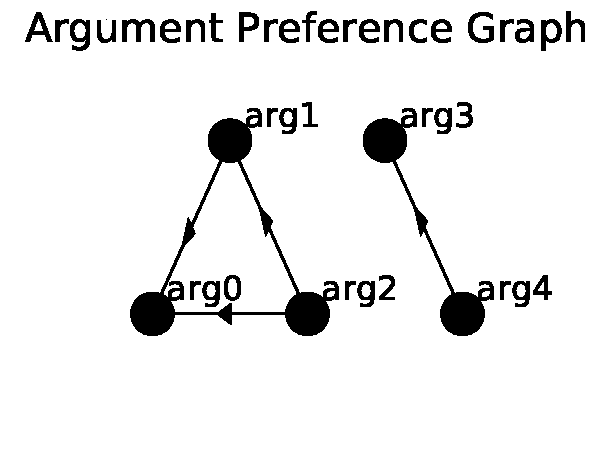
\includegraphics[width=0.5\columnwidth, clip=True, trim=30 30 20 30]{figures/cycles_demo/no_cycle/arggraph_arg_graph}
}
\subfloat[single cycle]{
  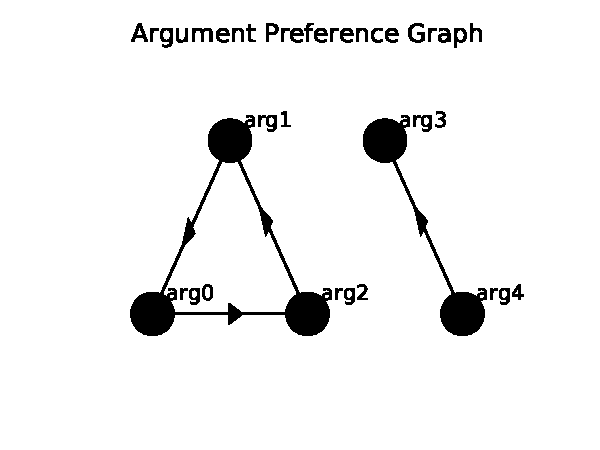
\includegraphics[width=0.5\columnwidth, clip=True, trim=30 30 20 30]{figures/cycles_demo/simple_cycle/arggraph_arg_graph}
}
\subfloat[double cycle]{
  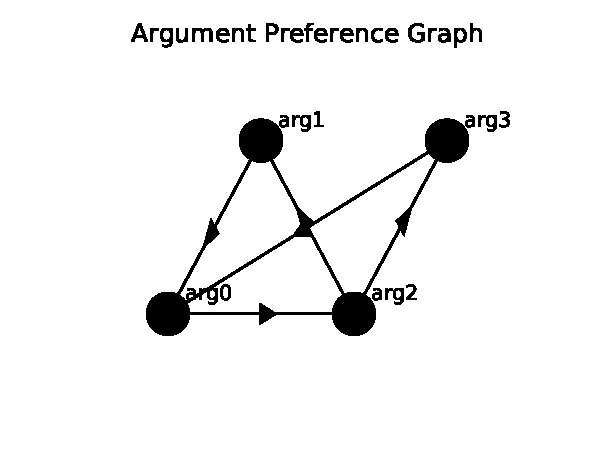
\includegraphics[width=0.5\columnwidth, clip=True, trim=30 30 20 30]{figures/cycles_demo/double_cycle/arggraph_arg_graph}
}
\subfloat[cycle with 9 undecided prefs.]{
  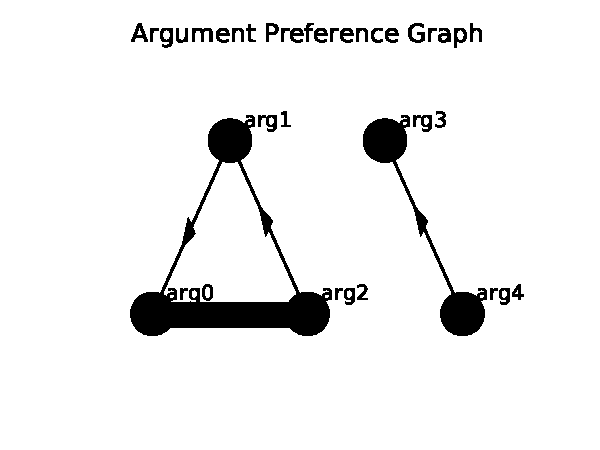
\includegraphics[width=0.5\columnwidth, clip=True, trim=30 30 20 30]{figures/cycles_demo/undecided/arggraph_arg_graph}
}
}\\
\subfloat[Ranking scores for arguments (bars for GPPL show standard deviation of latent preference function)]{ 
\label{fig:scores}
  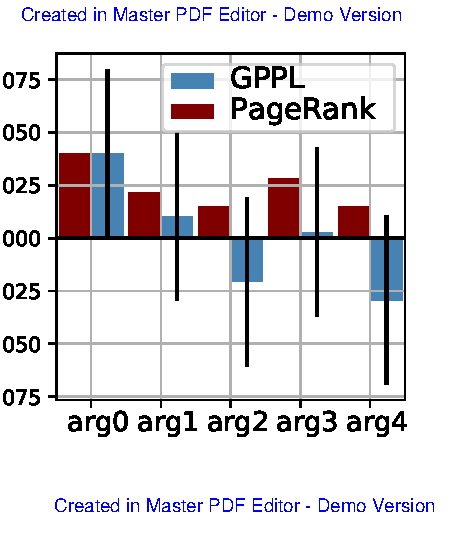
\includegraphics[width=0.5\columnwidth, clip=True, trim=20 5 10 22]{figures/cycles_demo/no_cycle/PageRank_scores}
%}
%\subfloat[]{ 
  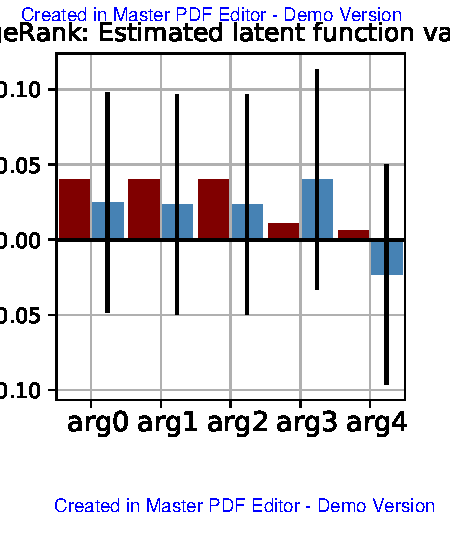
\includegraphics[width=0.5\columnwidth, clip=True, trim=20 5 10 22]{figures/cycles_demo/simple_cycle/PageRank_scores}
%}
%\subfloat[]{ 
  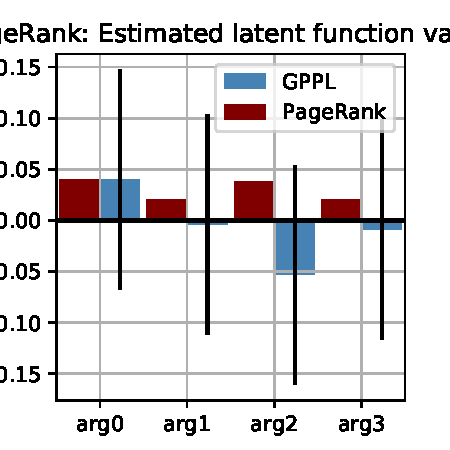
\includegraphics[width=0.5\columnwidth, clip=True, trim=20 5 10 22]{figures/cycles_demo/double_cycle/PageRank_scores}
%}
%\subfloat[]{ 
  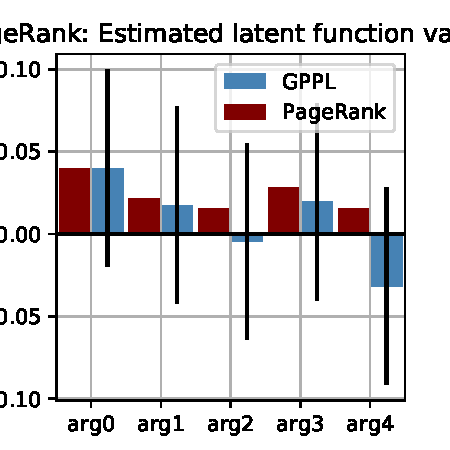
\includegraphics[width=0.5\columnwidth, clip=True, trim=20 5 10 22]{figures/cycles_demo/undecided/PageRank_scores}
}\\
\subfloat[GPPL predictions: probability that the argument 
on the horizontal axis is preferred to the argument on the vertical axis.]{
\label{fig:gppl_classifications}
  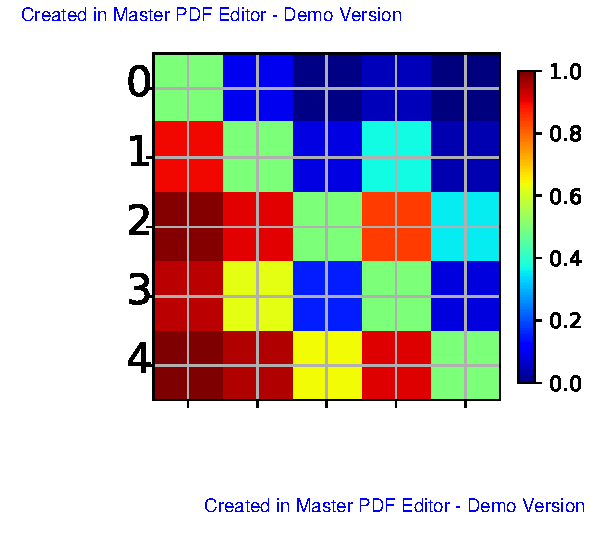
\includegraphics[width=0.49\columnwidth, clip=True, trim=58 5 41 24]{figures/cycles_demo/no_cycle/GPPL_probas}
%}
%\subfloat[]{
  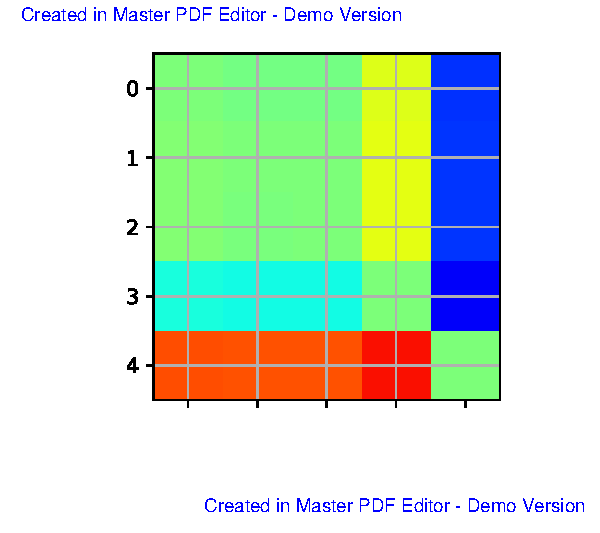
\includegraphics[width=0.49\columnwidth, clip=True, trim=58 5 41 24]{figures/cycles_demo/simple_cycle/GPPL_probas}
%}
%\subfloat[]{
  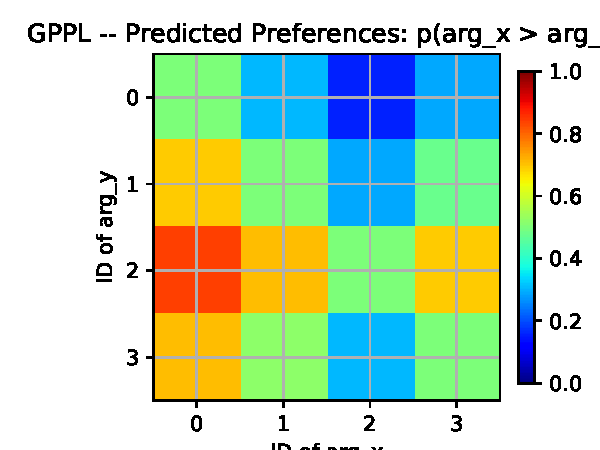
\includegraphics[width=0.49\columnwidth, clip=True, trim=58 5 41 24]{figures/cycles_demo/double_cycle/GPPL_probas}
%}
%\subfloat[]{
  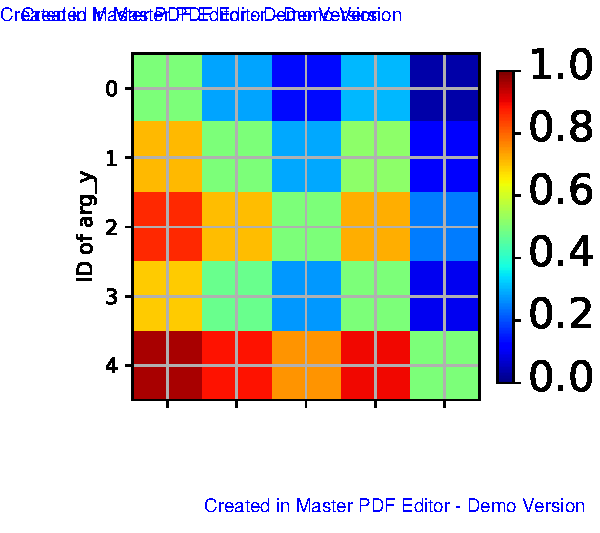
\includegraphics[width=0.56\columnwidth, clip=True, trim=58 5 10 24]{figures/cycles_demo/undecided/GPPL_probas}
}\\
\subfloat[SVM predictions: probability that the argument 
on the horizontal axis is preferred to the argument on the vertical axis.]{
\label{fig:svm_classifications}
  \includegraphics[width=0.49\columnwidth, clip=True, trim=58 5 41 24]{figures/cycles_demo/no_cycle/SVM_probas} 
%}
%\subfloat[]{
  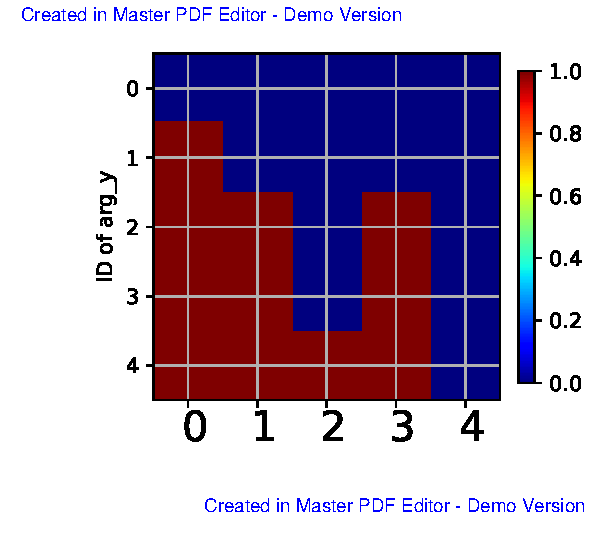
\includegraphics[width=0.49\columnwidth, clip=True, trim=58 5 41 24]{figures/cycles_demo/simple_cycle/SVM_probas} 
%}
%\subfloat[]{
  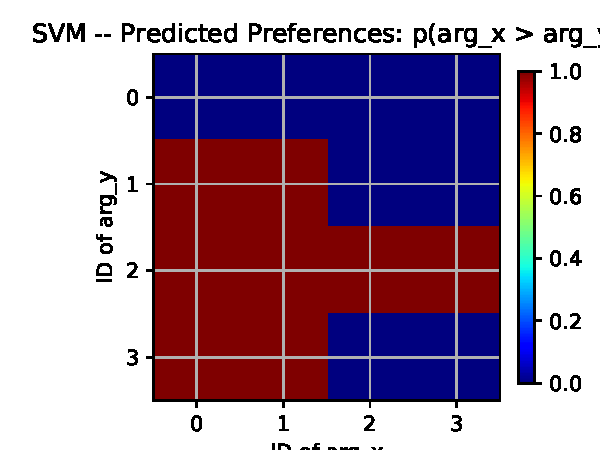
\includegraphics[width=0.49\columnwidth, clip=True, trim=58 5 41 24]{figures/cycles_demo/double_cycle/SVM_probas} 
%}
%\subfloat[]{
  \includegraphics[width=0.56\columnwidth, clip=True, trim=58 5 10 24]{figures/cycles_demo/undecided/SVM_probas} 
}
\caption{Preference graphs and predictions for simulated arguments in different scenarios. The plots in each column correspond to a single scenario.}
\end{figure*}

\subsection{Experiment 2: Clean Data}
\todo{emphasise we beat state of the art}
\todo{what kind of error analysis is required? Review other papers on similar topics (see comments in latex source).
%From semantic role labelling EACL paper: "In order to verify that this and argu- ment filler clustering were not the only aspects of our approach contributing to performance im- provements, we also evaluated our coupled model without Brown clustering and treating modifiers as regular arguments". "Due to the space con- straints we are not able to present detailed anal- ysis of the induced similarity graph D, however, argument-key pairs with the highest induced sim- ilarity encode, among other things, passivization, benefactive alternations, near-interchangeability of some subordinating conjunctions and preposi- tions (e.g., if and whether), as well as, restoring some of the unnecessary splits introduced by the argument key definition (e.g., semantic roles for adverbials do not normally depend on whether the construction is passive or active)."
%From what makes a convincing argument: "some topics are more challenging regardless of the system", "We examined about fifty random false predic- tions to gain some insight into the limitations of both systems. We looked into argument pairs, in which both methods failed, as well as into instances where only one model was correct. BLSTM won in few cases by properly catching jokes or off-topic arguments; SVM was properly catching all-upper-case arguments (considered as less convincing). By examining failures common to both systems, we found several cases where the prediction was wrong due to very negative senti- ment (which might be a sign of the less convinc- ing argument), but in other cases an argument with strong negative sentiment was actually the more convincing one. In general, we did not find any tendency on failures; they were also independent of the worker assignments distribution, thus not caused by likely ambiguous (hard) instances." --> i.e. only half a column
%of text is needed. 
% From Semantic Annotation Aggregation with Conditional Crowdsourcing Models and Word Embeddings (about half a page): ""
Where do the models differ?
}
\todo{
Note that human upper bound is 93\% so we could still improve (with better background knowledge?)
}
\todo{statistical significance?}
We comparemethods for classification on the UKPConvArgStrict dataset and ranking on the UKPConvArgRank dataset. 
Both datasets were cleaned to remove disagreements between annotators as stated in Table \ref{tab:expt_data}
To choose settings for the GPPL hyper-parameters $a_0$ and $b_0$, which control
the noise variance, we tested three different settings and found $a_0=2$, $b_0=200$
to be most effective. This is a weak prior favouring a moderate level of noise.
% We also tested $a_0=1$, $b_0=1$, which favours lower noise variance, but this resulted in
% a cross entropy error (CEE) of $0.69$ because the predicted classifications were very close to $0.5$, compared to CEE of $0.47$ when using $a_0=2$, $b_0=200$. With stronger
% priors $a_0=2e3$, $b_0=2e5$, we observed a drop in accuracy of $7\%$ on UKPConvArgStrict so concluded that $a_0=2$, $b_0=200$ is a reasonable setting to proceed without further optimisation.
To set the length-scale for GPPL, we compare the median heuristic (labelled ``medi.")
with the MLII optimisation method (labelled as ``OptGPPL").
We also compare multiplicative and additive combinations for the kernel functions for each feature.
We tested GPPL with different sets of input features:
~32000 linguistic features labelled as \emph{ling}, which 
we also use for SVM, as in Habernal and Gurevych~\shortcite{habernal2016argument});
\emph{Glove} word embeddings with 300 dimensions, which we also use for BLSTM, also as in Habernal and Gurevych~\shortcite{habernal2016argument};
and the combination of both lin and Glove embeddings (\emph{ling+Glove}). 
To create a single embedding per argument as input for GPPL,
we take the mean of the individual word embeddings for the tokens in the argument.

%\begin{enumerate}
%  \item Which type of kernel combination is most effective for GPPL? We compare with both heuristic length-scale and optimized, in case the heuristic is poor for one of the kernel combinations. Result: little difference between additive and multiplicative kernels over the features. GP methods are heavily affected by choice of kernel. The standard approach (using a product of kernels for each feature) is equivalent to taking the euclidean distance between points in feature space. These distances become very large when we have a large number of features. Each point needs to be close in all dimensions in order to be close overall. An alternative to this product kernel is to use a sum kernel, which will result in points having strong covariance if some (rather than all) features are similar. This may be suitable for high-dimensional settings where some features may have missing values. Compare the GPPL approach with product and sum kernels. 
%  \item Besides the choice of kernel itself, another important set of hyperparameters of the GPPL are the hyperparameters for the prior over the output scale of the kernel. The output scale controls the noise of the preferences, and needs to be large enough to allow the posterior to deviate substantially from the prior mean given only a small number of observations at each point. We test three different plausible settings of this hyperparameter to determine how sensitive the results are. Result: heavily informative values do not work well; very noninformative values are effective, although we observe a small boost when using an intermediate setting. This may be due to the data sparsity; the intermediate setting puts more weight onto each individual observation.
%\end{enumerate}

%% IMportant results have been merged into 2
%\begin{table}
%  \begin{tabularx}{\columnwidth}{ | l | X |  X |  X |  X | X| X|} \hline
%\multicolumn{7}{| l |}{UKPConvArgStrict} \\   \hline
% & \multicolumn{4}{|l|}{median heuristic} & \multicolumn{2}{|l|}{ARD} \\ 
%Kernel: & + & \multicolumn{3}{ l |}{*} & + & *\\ 
%$a_0$:  & 2    & 2    & 1    & 2e3 & 2 & 2\\ \hline
%$b_0$:  & 200  & 200  & 1    & 2e5 & 200 & 200 \\ \hline
%\\ \hline
%Acc.:   & 0.78 & 0.79 & 0.80 & 0.72  & ? & 0.80\\
%AUC:    & 0.86 & 0.87 & 0.87 & 0.79 & ? & 0.87 \\
%CEE:    & 0.69 & 0.47 & 0.69 & 0.39 & ?  & 0.51 \\
%\hline \multicolumn{7}{| l |}{UKPConvArgRank} \\   \hline
%Pears.: & 0.40 & 0.45 & 0.43 & - & ?  & 0.44 \\
%Spear.: & 0.64 & 0.65 & 0.67 & - & ? & 0.67 \\
%Kend.:  & 0.49 & 0.49 & 0.50 & - & ? & 0.50 \\
%\hline
%  \end{tabularx}
%  \caption{Different hyper-parameters and kernel combinations for 
%  GPPL with Glove + ling features}
%\end{table}
\todo{Remove discussion of different kernels and just show best}
The results are shown in Table \ref{tab:clean_results}. When using \emph{ling} features,
GPPL produces similar accuracy and improves the area under the ROC curve (AUC) by 2\%,
and cross entropy error by 0.01. Much larger improvements can be seen in the ranking metrics. 
When GPPL is run with mean Glove embeddings, it performs worse than
BLSTM for classification but improves the ranking metrics. Using a combination of features,
GPPL performs substantially better than the alternative methods for both classification and
ranking, suggesting that embeddings and linguistic features contain complementary information.
Optimising the length-scale using Bayesian model selection improves performance by 2\% over the median heuristic. 
However, the cost of these improvements is that each fold required around 2 hours to compute instead of approximately 10 minutes on the same machine (an Intel i7 quad core desktop) using the median heuristic. 
While there is an improvement in then mean accuracy with length-scale optimisation, 
the accuracy does not improve for every fold.
% is shown in Table \ref{tab:opt_by_fold}, and shows that optimisation does not always improve performance. 
Since the optimisation step is performed using only the training folds and the model is tested 
on a different topic, there is a possibility of overfitting: features that are important in the 
test fold may not appear relevant in the training folds. 
% Optimisation may therefore be more effective if it could be 
% executed in a semi-supervised manner by including unlabelled data from the target topic.

We hypothesised that GPPL benefits from integrating the GP to learn the latent preference function
directly from the discrete noisy preference labels. 
We compare GPPL against a two stage method shown in Table \ref{tab:clean_results} as \emph{PL+SVR}: 
first, we use use the GPPL preference likelihood method without any item features to infer convincingness scores for each argument from the pairwise labels; 
second, we perform SVM regression on the inferred scores with \emph{ling+Glove} features.
The results show that PL+SVR does not reach the same performance as GPPL. 
This suggests that GPPL benefits not just from its preference likelihood but also from
the integration of the GP.

For the pairwise classification task, we also compare GPPL against a Gaussian process classifier (\emph{GPC}) to investigate whether other GP-based approaches produce comparable performance. As shown in Table \ref{tab:clean_results}, GPC produces the best results on the classification task, although it cannot be used
to rank the arguments.
While the classification approach involves learning over twice as many features -- the features of the first and second items in each pair are concatenated -- the GPC may perform better on this dataset 
because it is trained directly on the classification task, rather than through a preference learning likelihood. 
% However, while this demonstrates some benefits of GP approach, the GPC cannot readily be used for ranking arguments.
%\begin{enumerate}
%  \item Compare GP preference learning (GPPL) to SVM using linguistic features. Result: better performance on ranking tasks.
%  \item Compare GPPL to Bi-LSTM. Result: GPPL is not as effective with mean embeddings, but GPPL with linguistic features still outperforms Bi-LSTM on all metrics.
%  \item Do the embeddings and linguistic features provide complementary information? Run GPPL with both sets of features. Result: improvement on classification tasks; larger improvement on ranking; suggests that the feature sets contain complementary information. The computational cost (of kernel computation, which dominates the overall cost in these experiments) grows linearly with number of features.
%  \item Does GPPL improve ranking performance because of the preference likelihood, or the way it makes predictions? Compare against feature-free preference learning used to train an SVM regression model (PL+SVR). Result: GPPL improves classification slightly on noise-free dataset, and improves more over PL+SVR on ranking and noisy classification tasks. GPPL resolves conflicts at the same time as predicting scores using similarities between arguments in feature space, so therefore has more information to resolve erroneous labels than the feature-free PL.
%  \item Performance improvements may be down to using a Bayesian approach with sparse data. Can we improve 
%  classification performance by training a GP Classifier rather than using GPPL? The feature space is increased by 
%doing this. Result: improvements on strict dataset but not when there is more noise. Maybe a downside of increased 
%sparsity meaning that erroneous points are further away from any correct points that would resolve the problems? 
%  \item What is the benefit of length-scale optimisation for GPPL versus our heuristic length-scale estimates? 
%Result: there is a performance improvement but it is not completely consistent (can overfit) and it comes at a 
%large cost. Therefore, our other comparisons will use the heuristic length-scales unless stated.  
%\end{enumerate}
\begin{table*}
  \begin{tabularx}{\textwidth}{ | l  | X |  X |  X |  X |  X | X | X | X | X | X |}
  \hline
\multicolumn{11}{| l |}{UKPConvArgStrict} \\   \hline
       &SVM  &BLSTM&\multicolumn{3}{c|}{GPPL*, medi.}&GPPL*, opt & GPPL+, medi. & GPPL+, opt & PL +SVR    & GPC \\\hline
       &ling &Glove  &ling &Glove &\multicolumn{6}{c|}{ling+ Glove}\\\hline
Acc.:  &0.78 &0.76   &0.78 &0.71  &0.79  & 0.80  & 0.78 & 0.78  & 0.78  & 0.81 \\
AUC:  &0.83 &0.84   &0.85 &0.77  &0.87  & 0.87 & 0.86  &  0.86 & 0.85  & 0.89 \\
CEE:   & 0.52 &0.64  &0.51 &1.12  &0.47  & 0.51 & 0.69  & 0.69 & 0.51  & 0.43 \\
\hline \multicolumn{11}{| l |}{UKPConvArgRank} \\   \hline
Pears.:&0.36&0.32   &0.38 &0.33  &0.45  &  0.44 & 0.40 &  0.40 & 0.39  & - \\
Spear.:&0.47&0.37   &0.62 &0.44  &0.65  &  0.67 & 0.64 &  0.64 & 0.63  & - \\
Kend.: &0.34&0.27&0.47 &0.31  &0.49     &  0.50 & 0.49 &  0.49 & 0.47  & - \\
\hline
  \end{tabularx}
  \caption{Performance comparison on clean datasets. }
  \label{tab:clean_results}
\end{table*}
\todo{Remove results for different kernels and just show best}
% \begin{table}
% \npdecimalsign{.}
% \nprounddigits{2}
% \npnoaddmissingzero
%   \begin{tabularx}{\columnwidth}{ p{3.2cm}  | p{1.7cm} | n{0}{2} | n{0}{2} }
%  Topic & Stance & {M.H.} & {Opt.} \\
% \hline\hline
% \multirow{ 2}{*}{\parbox{ 3.2cm}{Ban plastic water bottles?}} & no & .8125 & .80902778\\
% & yes & .83 & .8825 \\ \hline
% 
% \multirow{ 2}{*}{\parbox{ 3.2cm}{Christianity or atheism?}} & atheism & .82874618 & .81345566\\
%  & Christianity & .78076923 & .76923077\\ \hline
% 
% \multirow{ 2}{*}{\parbox{ 3.2cm}{Evolution vs creation}} & creation & .86516854 & .88764045\\
% & evolution & .72941176 & .72\\ \hline
% 
% \multirow{ 2}{*}{\parbox{ 3.2cm}{Firefox vs Internet Explorer}} & IE & .8649635  & .83576642\\
% & firefox & .86708861 & .85864979\\ \hline
% 
% \multirow{ 2}{*}{\parbox{ 3.2cm}{Gay marriage -- right or wrong?}} & right & .77722772 & .76237624\\
% & wrong & .86353468 & .90380313\\ \hline
% 
% \multirow{ 2}{*}{\parbox{ 3.2cm}{Should parents use spanking?}} & no & .8543956  & .84615385\\
% & yes& .72619048 & .68452381\\ \hline
% 
% \multirow{ 2}{*}{\parbox{ 3.2cm}{If your spouse committed murder...}} & no & .6686217  & .68914956\\
% & yes & .76011561 & .72254335\\ \hline
% 
% \multirow{ 2}{*}{\parbox{ 3.2cm}{India has the potential to lead the world}} & no & .82493369 & .78249337\\
% & yes & .84116331 & .81879195\\ \hline
% 
% \multirow{ 2}{*}{\parbox{ 3.2cm}{Lousy father better than fatherless?}} & no & .79166667 & .75694444\\
% & yes & .69604863 & .64741641\\ \hline
% 
% \multirow{ 2}{*}{\parbox{ 3.2cm}{Is porn wrong?}} & no & .80174927 & .81049563\\
% & yes & .88596491 & .88596491\\ \hline
% 
% \multirow{ 2}{*}{\parbox{ 3.2cm}{School uniform -- good or bad idea}} & bad & .84597701 & .82528736\\
% & good & .73863636 & .80454545\\ \hline
% 
% \multirow{ 2}{*}{\parbox{ 3.2cm}{Pro choice vs pro life}} & pro choice & .69411765 & .71294118\\
% & pro life & .84486874 & .79952267\\ \hline
% 
% \multirow{ 2}{*}{\parbox{ 3.2cm}{Should physical edu. be mandatory?}} & yes & .82865169 & .86797753\\
% & no & .72169811 & .75\\ \hline
% 
% \multirow{ 2}{*}{\parbox{ 3.2cm}{TV is better than books}} & no & .81412639 & .81412639\\
% & yes & .82045929 & .87056367\\ \hline
% 
% \multirow{ 2}{*}{\parbox{ 3.2cm}{Personal pursuit or common good?}} & common & .77984085 & .70822281\\
% & personal & .65633803 & .67042254\\ \hline
% 
% \multirow{ 2}{*}{\parbox{ 3.2cm}{Farquhar the founder of Singapore?}} & no & .81473214 & .80357143\\
%  & yes & .82573727 & .65951743\\ \hline\hline
%  
%  Average & & .79 & .80 
%   \end{tabularx}
%   \caption{Breakdown of accuracy by fold (topic and stance) for GPPL with different 
%   methods of choosing the length-scale (M.H. = median heuristic, Opt. = optimised).}
%   \npnoround
%   \npaddmissingzero
%   \label{tab:opt_by_fold}
% \end{table}

\subsection{Experiment 3: Conflicts and Noisy Crowdsourced Data}

\todo{Can we crunch expt 2 and 3 together? Perhaps 3 can be dropped entirely so we make the same point with active learning.}
In this experiment, we introduced 
%conflicts into the classification task by comparing methods on the UKPConvArgAll dataset, then additionally introduce 
noise to both the classification and the regression tasks by 
comparing on the UKPConvArgCrowdSample dataset.
Our goal was to investigate whether a Bayesian approach is better able to handle noise and conflicts. 

The results are shown in Table \ref{tab:noisy}, showing that all methods perform worse
when there are noisy or conflicting preferences. 
GPPL and GPC produce the best results, but GPC no longer has a clear advantage over GPPL. 
GPPL now outperforms the other methods in all metrics except Spearman's $\rho$, where PL+SVR performs slightly better. 
It is possible that GPC and SVM have the
largest changes in accuracy compared to the UKPConvArgStrict results because these classification-based methods
have no mechanism to resolve conflicts in the preference graph. The performance of the BLSTM classifier also 
decreases by a smaller amount, but was already poorer than the other methods on UKPConvArgStrict so it is hard to 
compare this change directly. PL+SVR is again slightly poorer than GPPL and GPC.
%When noise is introduced in the UKPConvArgCrowdSample dataset, most results drop further. 
% The accuracy of GPC and SVM decreases, as a result of the noise that was introduced,
% while for other methods it remains the same as for UKPConvArgAll. 
Metrics for ranking on UKPConvArgCrowdSample show that while GPPL and PL+SVR continue to perform well, the 
results for BLSTM and particularly for SVM are much poorer than with UKPConvArgRank. 

% \begin{enumerate}
%   \item How much does performance drop when we allow conflicts in the preference graph? Compare GPPL, SVM, Bi-LSTM. Result: all methods have a small drop in performance, but GPPL is affected least.
%   \item How much does performance drop if we use noisy crowdsourced labels, rather than the gold standard produced by MACE? Compare GPPL, SVM, Bi-LSTM. Result: as in previous experiment, GPPL copes best with the added noise. 
% \end{enumerate}

\begin{table}
  \begin{tabularx}{\columnwidth}{ | l | X | X | X | X | X |}\hline
% \multicolumn{6}{|l|}{UKPConvArgAll} \\   \hline
             & SVM &B-LSTM &GPPL         &PL+ SVR     &GPC \\
             &ling &Glove & ling+ Glove &ling+ Glove&ling+ Glove\\\hline
% Acc:     &0.71 &0.73  & 0.77        &0.75       &0.76 \\
% AUC:          &0.81 &0.81  & 0.84        &0.82       &0.86 \\
% CEE:          &0.56 &0.53  & 0.49        &0.52       &0.50 \\
\hline \multicolumn{6}{| l |}{UKPConvArgCrowdSample} \\   \hline
Acc:     &0.70 &0.73  & 0.77        &0.75       &0.73 \\
AUC:          &0.81 &0.80  & 0.84        &0.82       &0.86 \\
CEE:          &0.58 &0.54  & 0.50        &0.55       &0.53 \\
Pears.:      &0.06 &0.26  & 0.35        &0.31       & - \\
Spear.:     &0.04 &0.20  & 0.54        &0.55       & - \\
Kend.:      &0.04 &0.13  & 0.40        &0.40       & - \\
\hline
  \end{tabularx}
  \caption{Performance comparison on datasets containing conflicts and noise.}
  \label{tab:noisy}
\end{table}

\subsection{Experiment 4: Active Learning}

We hypothesised that a Bayesian approach would deal better with sparse data and provide more meaningful confidence estimates. To test this hypothesis, we simulated an active learning scenario, in which we simulate an agent that
iteratively learns a model for each fold. Initially, $N_{inc}=2$ pairs were chosen at random from the training set,
then used to train the classifier. The agent then performs \emph{uncertainty sampling} to select the $N_{inc}=2$
 pairs with the least confident classifications. The labels for these pairs are then taken from the training set and 
used to re-train the model. The result is plotted in Figure \ref{fig:active_learning}, showing that GPPL
is able to reach accuracies above 65\% with only 50 labels, while SVM and BLSTM do not reach the same performance
given 200 labels. The accuracy of GPPL also increases by approximately 8\% given 200 labels, while SVM increases
approximately 6\% and BLSTM only 2\%. This suggest that GPPL may be a more suitable model to be used with
uncertainty sampling in situations where obtaining labelled data is expensive.
\begin{figure}
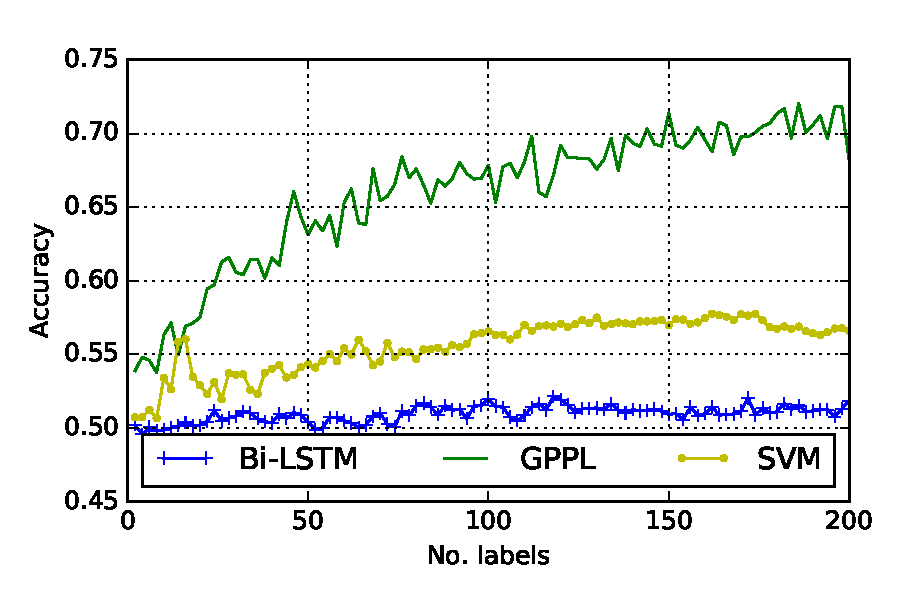
\includegraphics[width=1.0\columnwidth,trim=0 0 0 22,clip=true]{figures/active_learning/test_acc}
\caption{Active learning simulation for the three methods showing the mean accuracy of preference pair classifications over 32 runs.}
\label{fig:active_learning}
\end{figure}

% This plot is invalid because SVM and BLSTM are trained on the output from PageRank with all the data!
% \begin{figure}
% 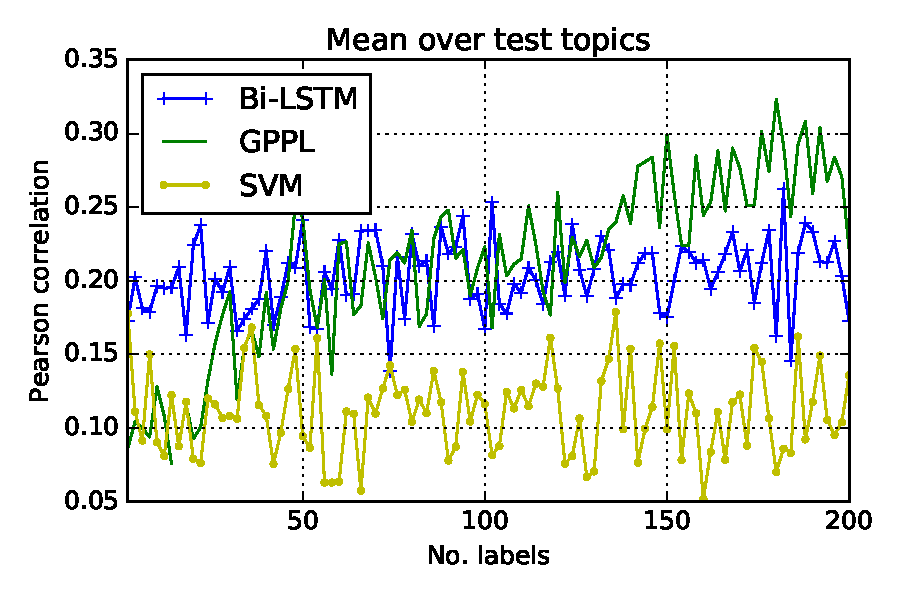
\includegraphics[width=1.0\columnwidth,trim=0 0 0 23,clip=true]{figures/active_learning/test_pearson}
% \caption{Active learning simulation for the three methods showing the mean pearson correlation with the gold standard ranking over 32 runs.}
% \end{figure}

\subsection{Experiment 5: Embeddings}

\todo{cut this section and just state that we found no improvement with other embeddings?}
In our previous experiments, we found that including mean Glove word embeddings boosted performance above only using linguistic features. However, there are several alternative methods to mean word embeddings for representing longer pieces of text, 
notably skip-thoughts~\cite{kiros2015skip} and Siamese-CBOW~\cite{kenter2016siamesecbow}.
We compare mean Glove embeddings with skip-thoughts embeddings 
and Siamese-CBOW and show the results in Table \ref{tab:embeddings}. 
The best performance
was obtained using mean Glove embeddings, despite the simplicity of this approach.
Further work may be required to assess whether skip-thoughts and Siamese-CBOW 
can be improved if trained on different corpora.
% whether the mean word embeddings
%are simply more informative for predicting convincingness on our chosen dataset.
% with both median heuristic length-scale and optimized length-scale to ensure that %differences in performance are not caused by the heuristic failing with certain embedding %types. Result: awaiting optimized results, but non-optimized results show that word mean %was most effective.
%\end{enumerate}
% Could be merged into 2 and 3
\begin{table*}
  \begin{tabularx}{\textwidth}{ | l | X | X | X | X |  X |  X |  X | X | X |}
  \hline  \multicolumn{10}{| l |}{UKPConvArgStrict} \\   \hline
       & \multicolumn{6}{ l |}{Median heuristic}                                     & \multicolumn{3}{l|}{Optimised} \\
       &Glove &Skip-thoughts &SCBOW &ling+ Glove &ling+ Skip-th. &ling+ SCBOW &ling+ Glove &ling+ Skip-th. & ling+ SCBOW \\ \hline
Acc.:  & 0.71 & 0.67         & 0.69  & 0.79       & 0.74               & 0.77        & 0.80       & 0.78 & 0.78 \\
AUC:   & 0.77 & 0.72         & 0.75  & 0.87       & 0.81               & 0.85        & 0.87       & 0.85 & 0.85\\
CEE:   & 1.12 & 1.11         & 1.22  & 0.47       & 0.80               & 0.52        & 0.51       & 0.51 & 0.50\\
\hline \multicolumn{10}{| l |}{UKPConvArgRank} \\   \hline
Pears.:& 0.33 & 0.30         & 0.29  & 0.45       & 0.34               & 0.39        &   0.44     & 0.34 & 0.40\\
Spear.:& 0.44 & 0.49         & 0.40  & 0.65       & 0.59               & 0.63        &    0.67    & 0.52 & 0.63\\
Kend.: & 0.31 & 0.36         & 0.28  & 0.49       & 0.43               & 0.47        &    0.50    & 0.37 & 0.47\\
\hline
  \end{tabularx}
  \caption{Comparison between different types of embeddings with GPPL}
  \label{tab:embeddings}
\end{table*}
  \todo{remove results for different LS from table:embeddings}

\subsection{Experiment 6: Informative Features}

\todo{how much does this really show us? Could we skip this section to make more space for error analysis?
In contrast with Lampos et al 2014, we cannot identify a small number of important features --> looks like we need
a combination, perhaps a hierarchical feature representation.}
Finally, we show how the length-scales learned by optimising GPPL can be used to identify
informative sets of features. Since a larger length-scale causes greater smoothing, 
a very large length-scale implies that the value of that feature is irrelevant when predicting 
the function. In contrast, small length-scales indicate more informative features, since their
precise value affects the latent preference function.
Figure \ref{fig:boxplot} shows the distribution of optimised length-scales on one fold of UKPConvArgStrict. 
The values shown are ratios of the optimised value to the median heuristic. 
Due to the computation time required, our optimisation procedure was limited to $25$ function evaluations. 
The large number of values close to $1$ may be due to the L-BFGS-B
algorithm not being able to optimise all features in the available time, 
suggesting that other features with larger gradients were prioritised for optimisation
away from the median heuristic values. 
The length-scales for many dimensions of the mean word embeddings were increased,
giving ratios close to $4$ times the median heuristic, suggesting that these dimensions may be
only very weakly informative. Table \ref{tab:extreme_features} shows the largest
and smallest ratios for embeddings and linguistic features. The unigram "safety" has
a very high length-scale, suggesting it is not informative and may be discarded. 
% It is possible that continuing the optimisation procedure for a larger number of steps would 
% identify large length-scales for other features that may be discarded. However, caution is 
% required to avoid overfitting to the training set during optimisation~\cite{qi2004predictive}.
\begin{figure}
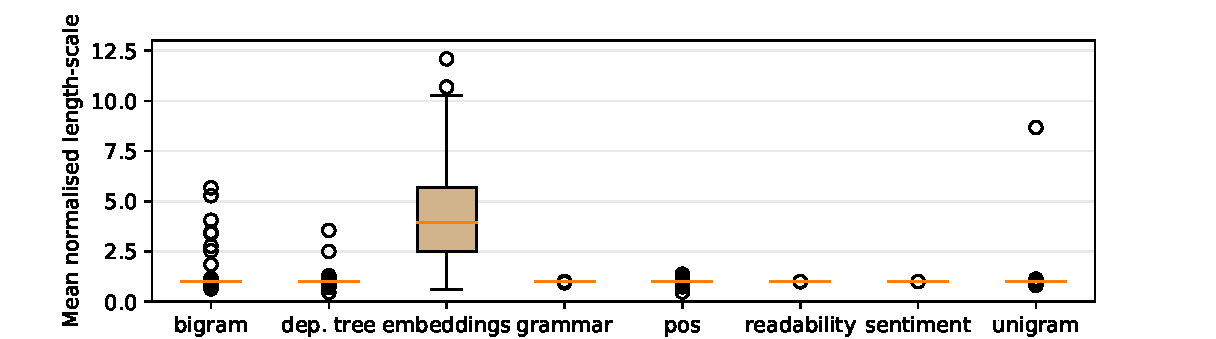
\includegraphics[width=\columnwidth, clip=True, trim=32 0 57 0]{figures/features/boxplot}
\caption{Distribution of length-scales for each type of feature after optimisation. 
Values are relative to the median heuristic value before optimisation, optimised 
on fold "should physical education be mandatory in schools -- no", where 
optimisation increased accuracy from 75\% to 80\%. }
\label{fig:boxplot}
\end{figure}
\begin{table}
  \begin{tabularx}{\columnwidth}{l | X }
  Feature & Ratio\\
  \hline
  ProductionRule-S-$>$ADVP,NP,VP,., & 0.466 \nonumber\\
  Pos-ngram-PP-O-CARD & 0.477 \nonumber\\
  Unigram-``safer", & 0.640 \nonumber\\
  \hline
  Bigram-``?"-``look" & 5.672 \nonumber\\
  Unigram-``safest" & 8.673 \nonumber\\
  Unigram-``safety" & 271.190 \nonumber\\
  \hline
  Embedding-dimension-19 & 0.610 \nonumber\\
  \hline
  Embedding-dimension-241 & 12.093 \nonumber\\
  \end{tabularx}
  \caption{Ratios of optimised to median heuristic length-scales: largest and smallest
  ratios for linguistic features and word embeddings.}
  \label{tab:extreme_features}
\end{table}


\subsection{Error Analysis}

We compared the errors when using GPPL with mean Glove embeddings
and with linguistic features. We
manually inspected the twenty-five arguments most frequently
mis-classified by GPPL \emph{ling} and correctly classified by GPPL \emph{Glove}.
We found that GPPL \emph{ling} mistakenly marked several arguments 
as less convincing where they contained grammar and spelling errors but otherwise
made a logical point. 
In contrast, arguments that did not strongly take a side but did not contain 
language errors were often marked mistakenly as more convincing.
We also examined the twenty-five arguments most frequently misclassified by GPPL \emph{Glove} and correctly labelled by GPPL \emph{ling}.
GPPL \emph{Glove} did not correctly mark arguments as less convincing 
even though they contained multiple exclamation marks and all-caps sentences. 
Other failures were very short arguments and underrating arguments containing the emotive term 'rape'.
The analysis confirms that the different feature sets can identify different aspects of convincingness.

% Notes on first paragraph:
% ling failed on:
% overrated: good grammar and structure but weak points?
% both; short and direct argument but not very thoughtful.
% both: seems well structured...
% both: seems to argue for middle ground rather than one side
% both: grammar/spelling errors but strong argument underneath?
% both: grammar/spelling errors but strong argument underneath?
% underrated: very specific example may seem off topic? 
% both: unclear points
% underrated: bad spelling but okay points
% underrated: very personal "I" language to make a good point
% mostly underrated: makes multiple points, some are quite extreme. 
% underrated: sounds quite personal "you" but strong argument.
% both: kind of doesn't try to convince strongly for one side although well written.
%  overrrated: doesn't address the main point although language is reasonable.
% mostly overrated: response to previous answer with no new points.
% underrated: contains '?' and 'you' a lot but makes a good point.
% overrated: language is reasonable, no mistakes, but doesn't clearly take a side.
% overrated: no obvious language indicators but doesn't address main point.
% underrated: lots of spelling mistakes hide the main point.
% mostly overrated: good language but doesn't really support or attack the point directly
% underrated argument with grammatical mistakes but possibly a good point?
% avoiding the argument/debate overrated
% illogical and quite emotional argument underrated
% personal/ad hom attack with 'crap' overrated -- but need to identify the username as such to know it  is a personal attack?
% obvious nonsense without proper words was overrated
%
% embeddings failed on:
%
% both: very short argument, unclear why ling features would help
% overrated: claims lack support
% overrated: spelling mistakes; doesn't address stance of the topic 
% underrated: very short; mean embedding could be an outlier?
% underrated: short
% underrated: no linguistic markers of a bad argument; unclear why embeddings a problem
%     mostly underrated; as above
% underrated: as above; perhaps the words such as 'rape' are associated in the embeddings
% with poor emotional arguments? Perhaps not the word 'rape' itself, but some of the related words in embedding space are common in bad arguments.
% underrated: no idea
% underrated: again mentions 'murder'
% mostly underrated: all caps; why underrated?
% underrated: sensible argument mentions 'personal' a lot
% underrated: very short; mentions wrong and right --> link to emotional arguments without evidence?
% overrated: very short and gives no argument; perhaps contains no bad argument embeddings but linguistic features such as word counts will show it up.
% overrated: mentions of 'dreamt'?
% underrated: no idea
% overrated: doesn't address main point; hard to see why ling would help
% underrated: no idea why; has no linguistic errors
% overrated: no idea; no idea why linguistic features help
% underrated: again maybe because of emotional topic of abortion; no linguistic problems
% overrated: very short sentence; no structure; lots of '!'
% overrated: grammatical errors, very short text that doesn't really make any point or provide any support
% overrated: nonsense detected by all caps
% overrated: very short, cannot really make a good point in that much text
% underrated: why this would beat any other argument is unclear; it's all caps and has lots of '!' too
% 
%  Problem is we don't see what they were misclassified against -- number of 
% misclassifications is too few to know if it is a general problem with that sentence.
% 
% which of these errors are resolved by combining? Pick out errors from either ling that
% were fixed with both; pick our errors from embeddings that were fixed with both.

% when comparing 'both' to 'ling', most of the errors that are made by embeddings
% no longer appear -- those with all caps and '!' have gone. Differences are few.
% seem to be that poorly written arguments continue to be mis-classified.
% with 'both' to embeddings, some of the errors that ling made have gone, e.g. including 'lol'. The remaining ones are mainly those with good superficial structure/correct grammar
% but covering emotional topics. Suggests need for better trade-off between semantics/deeper understanding and linguistic indicators such as good grammar.

% this analysis also shows whether the errors are due to epistemic uncertainty given the features (small difference in 
% similarities between false/true labelled items) or if better training data would help (larger difference between 
% false/true similarities). If GPPL handles the sparse data better, the difference should be reduced compared to SVM.
% the text below is good but the results are not really worth reporting...
%We next investigate whether the Bayesian approach is better able to handle sparsity in the training data. 
%Training data sparsity occurs when the training provides very few examples of arguments in some important regions of feature space, meaning  
% there are arguments in the test dataset that are not similar to any training arguments.
%For each fold, we computed the mean cosine similarity of each argument in the 
%test dataset to the arguments in the training dataset, which we refer to as \emph{training similarity}.
%For UKPConvArgStrict, the mean training similarity for the arguments in pairs correctly classified by GPPL (ling + Glove) was 694.63 and the mean for incorrectly classified arguments was 694.703. This suggests that training similarity is not a strong indicator of a correct
%prediction and training data sparsity does not appear to be a key source of error for GPPL
%in this dataset. In comparison, using  SVM,  
%the mean training similarity for correctly classified arguments
% was 694.72 against 0.     for incorrectly classified arguments, showing that 
% lower training data similarity corresponds to a more misclassified pairs. 
% This indicates that SVM was more affected by training data sparsity.
% However, the small difference in similarities indicates that sparsity was not a problem here?
% The lower similarity of correctly labelled arguments with GPPL suggests it is able to handle more outlying arguments correctly. 
%results: 
% using matern covariance to determine similarity:
% SVM: correctly classified pairs: 694.715334 (STD 3.251511), incorrectly classified pairs: 694.164449 (STD 3.809051). 
% So similarity to training data is higher for correct pairs.
% GPPL: correctly classified pairs: 694.625999 (STD 3.213874), incorrectly classified pairs: 694.703252 (STD 3.580148).
% with cosine similarity:
%SVM For all folds: mean total_sim for correctly classified pairs: 0.998826 (STD 0.021547)
%SVM For all folds: mean total_sim for incorrectly classified pairs: 0.998770 (STD 0.025875)
%GPPL For all folds: mean total_sim for correctly classified pairs: 0.998825 (STD 0.021434)
%GPPL For all folds: mean total_sim for incorrectly classified pairs: 0.998770 (STD 0.026505)
% Using max similarity rather than mean (most similar training point) gives similar results.
% So similarity to training data is actually higher for incorrect pairs; for correct pairs it is lower than for SVM. 
% Suggests that similarity to training data (not being outliers) is less important for GPPL.

To investigate the differences between our best approach, GPPL opt. (ling+Glove), 
and the previous best performer, SVM, 
we manually examined forty randomly chosen false classifications, where one of 
either GPPL (ling+Glove) or SVM (also ling) was correct and the other was incorrect. 
We found that both SVM and GPPL falsely classified arguments when they were either very short or long and complex, suggesting deeper semantic or structural understanding of the argument may be required. However, SVM also made mistakes
where the arguments contained few verbs.
%We were not able to identify any common source of error for cases where both 
%methods produced errors. % required deeper semantic understanding and background knowledge of the topics involved
% to evaluate the validity of claims.
% Case 1: SVM right, GPPL wrong.
% underrated, short
% overrated, maybe SVM is right because it dislikes '!'
% underrated, less common language -- perhaps not learned?
% overrated, complex language
% underrated, short argument
% ...
% overrated, irrelevant but well written
% more long arguments with fairly sophisticated language and no obvious errors.
% some cases of arguments that do not take a strong position either way
% The number of errors are small -- could be noise rather than consistent problems with GPPL.
% Some arguments with mainly topic-specific words were misclassified by GPPL but not SVM.
%notable that there are lots of errors on the singapore topics
% Case 2: GPPL right, SVM wrong
% short arguments with few verbs
% long arguments with no obvious language errors and no emotional arguments.
% notable that lots of errors on the school uniform topics
We also compare the rankings produced by GPPL opt. (ling+Glove), 
and SVM on UKPConvArgRank, by examining the 20 largest deviations from the 
gold standard rank for each method. SVM underrated some arguments that GPPL did not where they contained
exclamation marks, common spelling errors (likely due to unigram or bigram features).
GPPL underrated short arguments with the ngrams ``I think", ``why?", and
``don't know". In these cases, the phrases were used in a rhetorical question 
rather than to state that the author was uncertain or uninformed; these case
may not be possible to distinguish given \emph{ling + Glove} features.
% Case 1: GPPL better, SVM worse
% svm underrated some arguments containing !, thankyou, lots of 'if'
% underrated: long argument, common spelling errors (unigrams usually correlated with bad arguments?), India, long and complex arguments, short arguments
% overrated: ('because' could be either over or underrated), mention of another website, 
% Hard to see pattern here because the arguments are very varied in length, grammatical standard; most are not using emotive terms.

% Case 2: SVM better, GPPL worse
% mistakes by GPPL: several short arguments containing "i think"... perhaps leading to a more neutral score than the other features suggest?
% 

% Case 3: GPPL's worst problems (including mistakes by SVM)
% an argument with lots of caps in was underrated
% argument with lots of short sentences (sometimes few verbs) is underrated. 
% underrated: "why?"
% underrated: "don't know" is a big indicator. These two suggest that the model needs a way to determine whether the "don't know" was used in a way that undermines the argument strength (admission of a lack of knowledge) or as a rhetorical device to say that an opposing viewpoint is nonsensical ("don't know why they would do x"). 

% Entropy for SVM correct/incorrect labels: 0.187555, 1.583709
% Entropy for GPPL correct/incorrect labels: 0.128872, 2.443407
% Shows better division between certain and uncertain predictions
A proposed advantage of GPPL is that it provides more meaningful uncertainty estimates. 
We examined whether the erroneous classifications correspond to more uncertain predictions
when using GPPL compared to SVM when both methods use the \emph{ling} features.
For UKPConvArgStrict, the mean Shannon entropy
of the pairwise predictions from GPPL 
was 0.129 for correct predictions and 2.443 for errors,
showing that on average, more confident predictions were less likely to lead to errors.
For SVM, the mean Shannon entropy was  0.188 for correct predictions and 
1.583 for incorrect.
The more extreme values for the GPPL predictions 
 suggest that the probabilities provided by GPPL were indeed more reflective of 
 the probability of error than those given by the SVM classifier.

% % the analysis below is possible only using the predictions for the training points; however we do not predict for
% % the provided training points?
% To judge whether the GPPL improvements in UKPConvArgCrowdSample are due to better
% handling of noisy labels, we examined whether annotations that disagreed with the 
% MACE gold label -- i.e. erroneous training labels -- led to erroneous predictions. 
% We chart the results of this error analysis in Table \ref{tab:noise_errors}.
% This shows that while arguments with erroneous training labels are more likely to 
% be incorrectly classified using both SVM and GPPL, the Bayesian approach is less susceptible
% to this error.
% \begin{table}
% \begin{tabularx}{\columnwidth}{| l | X | X | X | X | }
% \hline
% & \multicolumn{4}{c | }{\emph{Predictions}} \\
% & \multicolumn{2}{c|}{SVM} & \multicolumn{2}{c|}{GPPL} \\\hline
% \emph{Annotations}           & \emph{True} & \emph{False} & \emph{True} & \emph{False} \\
% Incorrect & & & &  \\
% Correct   & & & & \\
% \hline
% \end{tabularx}
% \caption{Coincidence of erroneous annotations and false predictions by pairwise classification methods.}
% \label{tab:noise_errors}
% \end{table}
